\documentclass{scrreprt}
\usepackage[utf8]{inputenc}
\usepackage[english,ngerman]{babel}
\usepackage{lscape}
\usepackage{eurosym}
\usepackage{amsmath}
\usepackage{graphicx} 
\usepackage[left=2cm,right=2cm,top=2cm,bottom=2cm,includeheadfoot]{geometry} 
\usepackage{enumerate}
\usepackage{hyperref}

\usepackage{scrpage2}\pagestyle{scrheadings}
\ohead{\today}
\begin{document}
\chapter{Einführung}
\section{Intension}
\label{intension}
Zur Bewertung der Qualität des Unterrichtes, wird die Aufmerksamkeit der Schüler verwendet, da zwischen beiden ein Zusammenhang besteht. Allerdings ist der Parameter Aufmerksamkeit recht schwierig zu erfassen, wodurch verschiedene Verfahren verwendet werden. Unter anderem Fragebögen die ein Schüler selbst ausfüllen sollen oder die Auswertung durch einen Beobachter der bewertet ob ein einzelner Schüler Aufmerksam (on-Task) oder nicht (off-Task) ist.\\
Für die Bewertung ob on/off-Task werden Kriterien festgelegt, wie Blickrichtung, Körperhaltung und Tätigkeit, dann wird die Person beobachtet wie diese sich verhält.\\
Bei der Videostudie zur Wirksamkeit des Unterrichtsprozesses \cite{aufmerksamkeit_Studie} wurden die Kriterien Blickkontakt zum legitimen Sprecher oder Objekt, Aktive Beteiligung an der Aufgabe, keine Ausübung anderer Tätigkeiten, keine Motorische Unruhe und keine Themenferne Kommunikation festgelegt. Dann wird immer in einem 1min Intervalle der Schüler beobachtet und bewertet. Sollte drei oder mehr Punkte erfüllen, gilt der Schüler als on-Task.\\
Diese Art der Auswertung ist recht einfach, allerdings gibt es Interpretationsfreiheiten, gerade bei den Bewertungen der Tätigkeiten, die von jedem Beobachter anders gewertet werden. Außerdem ist es sehr zeitintensiv, so werden alleine zum anschauen des Videos für jeden Schüler bei einer Klassen (30 Personen) 30 min gebraucht und sollte jeder Schüler mehrfach beobachtet werden entsprechend mehr.\\
Sollten recht wenige Zyklen durchgeführt werden, so wird das gesamte Verhalten eines Schülers in der Unterrichtsstunde mit nur wenigen beobachteten Minuten beschrieben, die Auswertung benötigt allerdings entsprechend weniger Zeit.\\
Durch eine zu geringe Auswertungsrate kann nur eine Aussage über den gesamten Unterricht gemacht werden und nicht über einzelne Übungen oder ähnliches, auch die Bewertung eines einzelnen Schülers ist nur schwer möglich.
\cite{aufmerksamkeit_Studie}
\section{Problemstellung}
\label{Problemstellung}
Ziel dieser Arbeit ist es, eine automatisierte Auswertung der Blickrichtung, einem der wichtigsten Indikatoren für gerichtete Aufmerksamkeit, auf einer ganzen Klasse zu bestimmen.
Die Messung soll den Unterricht möglichst wenig beeinträchtigen, wodurch hierfür üblicherweise verwendete Geräte, wie z.B. Eye-Tracking Brillen, nicht verwendet werden können.
Zum einen ist die Anschaffung einer großen Stückzahl dieser Geräte teuer und wurde bisher nur in wenigen speziell eingerichteten Laboratorien durchgeführt (TüDiLab \cite{TueDiLab}) Zum anderen sind die Geräte entweder Ablenkend (Brillen) oder schränken den Aktionsradius ein (Remote Tracker).
Wären wir in der Lage solch eine Auswertung mit nur einer einzigen Kamera durchführen zu können, so ist der Aufbau und die Aufnahmen auch für technische Laien durchführbar.\\
Diese Arbeit untersucht, wie weit es technisch möglich ist das Filmmaterial einer Kamera, das die gesamte Klasse aufzeichnet, Auszuwerten im Bezug auf Blickrichtungen bzw. Ausrichtung des Gesichts und mit welchen Einschränkungen und Genauigkeiten zu rechnen ist.\\
\cite{MAI_Verhaltensbeobachtung}
\section{Das Klassenzimmer - Umgebung des Eye-Tracking}
Die Anwendung ist für den Unterricht ausgelegt, wie in der Problemstellung \autoref{Problemstellung} beschrieben und soll diesen möglichst wenig beeinflusst, ergeben sich folgende Randbedingungen:
\begin{itemize}
\item Brillen, Kontaktlinsen und ähnliches sind bei den Probanden erlaubt, ebenso Frisuren, Make-up usw.
\item Die üblichen Bewegungen im Unterricht wie Sprechen, Kopfdrehungen usw. der Schüler sind gestattet.
\item Das Verfahren soll gleichzeitig auf Distanzen zwischen $2.5 - 8m$ zur Kamera auf einer Breite von $6m$ funktionieren.
\item Möglichst alle Blickrichtungen bzw. die Gesichtsorientierung der Schüler sollen so exakt wie möglich erfasst werden.
\end{itemize}
Ein deutsches Klassenzimmer soll laut Baden-Württembergischen Schulbauempfehlungen eine Grundfläche von $54-66m^2$ aufweisen für maximal 28-32 Schülern. Da noch die Tafel usw. beachtet werden muss ergibt sich einen Abstand von $2.5 - 8m$ zwischen Kamera und Schüler auf einer Breiten von $6m$, dabei befindet sich die Kamera in der Nähe der Tafel. Somit muss der Linsenwinkel mindestens $100^\circ$ betragen, damit alle im Bild sind, mit entsprechender Schärfentiefe.\\
Außerdem soll die Anwendung auf schon vorhanden Aufnehmen eines Unterrichtes arbeiten, die oben genannten Bedingungen erfüllen.\\
\cite{bauordung}
\subsection{Randbedingungen der Anwendung}
Zusätzlich werden folgende Annahmen gemacht, die sich vor allem auf die Sitzrodung der Schüler und die Umgebung beziehen.
\begin{itemize}
\item Die Szene ist innerhalb eines Gebäudes, mit ausreichend gleichmäßiger Beleuchtung.
\item Die Überführung zwischen Welt- und Kamerakoordinatensystem ist bekannt.
\item Die Kamera befindet sich vor der Klasse, so dass die Hauptblickrichtung der Schüler in Richtung Kamera verläuft.\\
Gleichzeitig kann die Kamera jedoch nicht ohne weiteres ganz zentral angebracht werden, da dieser Raum für den Unterricht (Tafel/Lehrer) benötigt wird.
\item Die Gesichter sind komplett sichtbar und nicht verdeckt durch andere Schüler oder von der Kamera abgewannt.\\
Eine Sitzrodung, wie sie hauptsächlich im Frontalunterricht üblich ist.
\end{itemize}
\section{Verwendete Eingabegeräte \& Bibliotheken}
\label{hardware}
 wurden verschiedenen Farbkameras eingesetzt.\\
\\
%\subsection{Auswirkung von Pixelrauschen}
%Durch Aufnahme eines Schwarzbildes der Actioncam zeigt sich, dass das Pixelrauschen recht hoch ist, siehe \autoref{img_noishight}. Das Rauschen hat keine Normalverteilung, sondern es besteht aus kleinen Bereiche, die den selben fehlerhaften Farbwert besitzen.
%\begin{figure}
%	\centering
%	\fbox{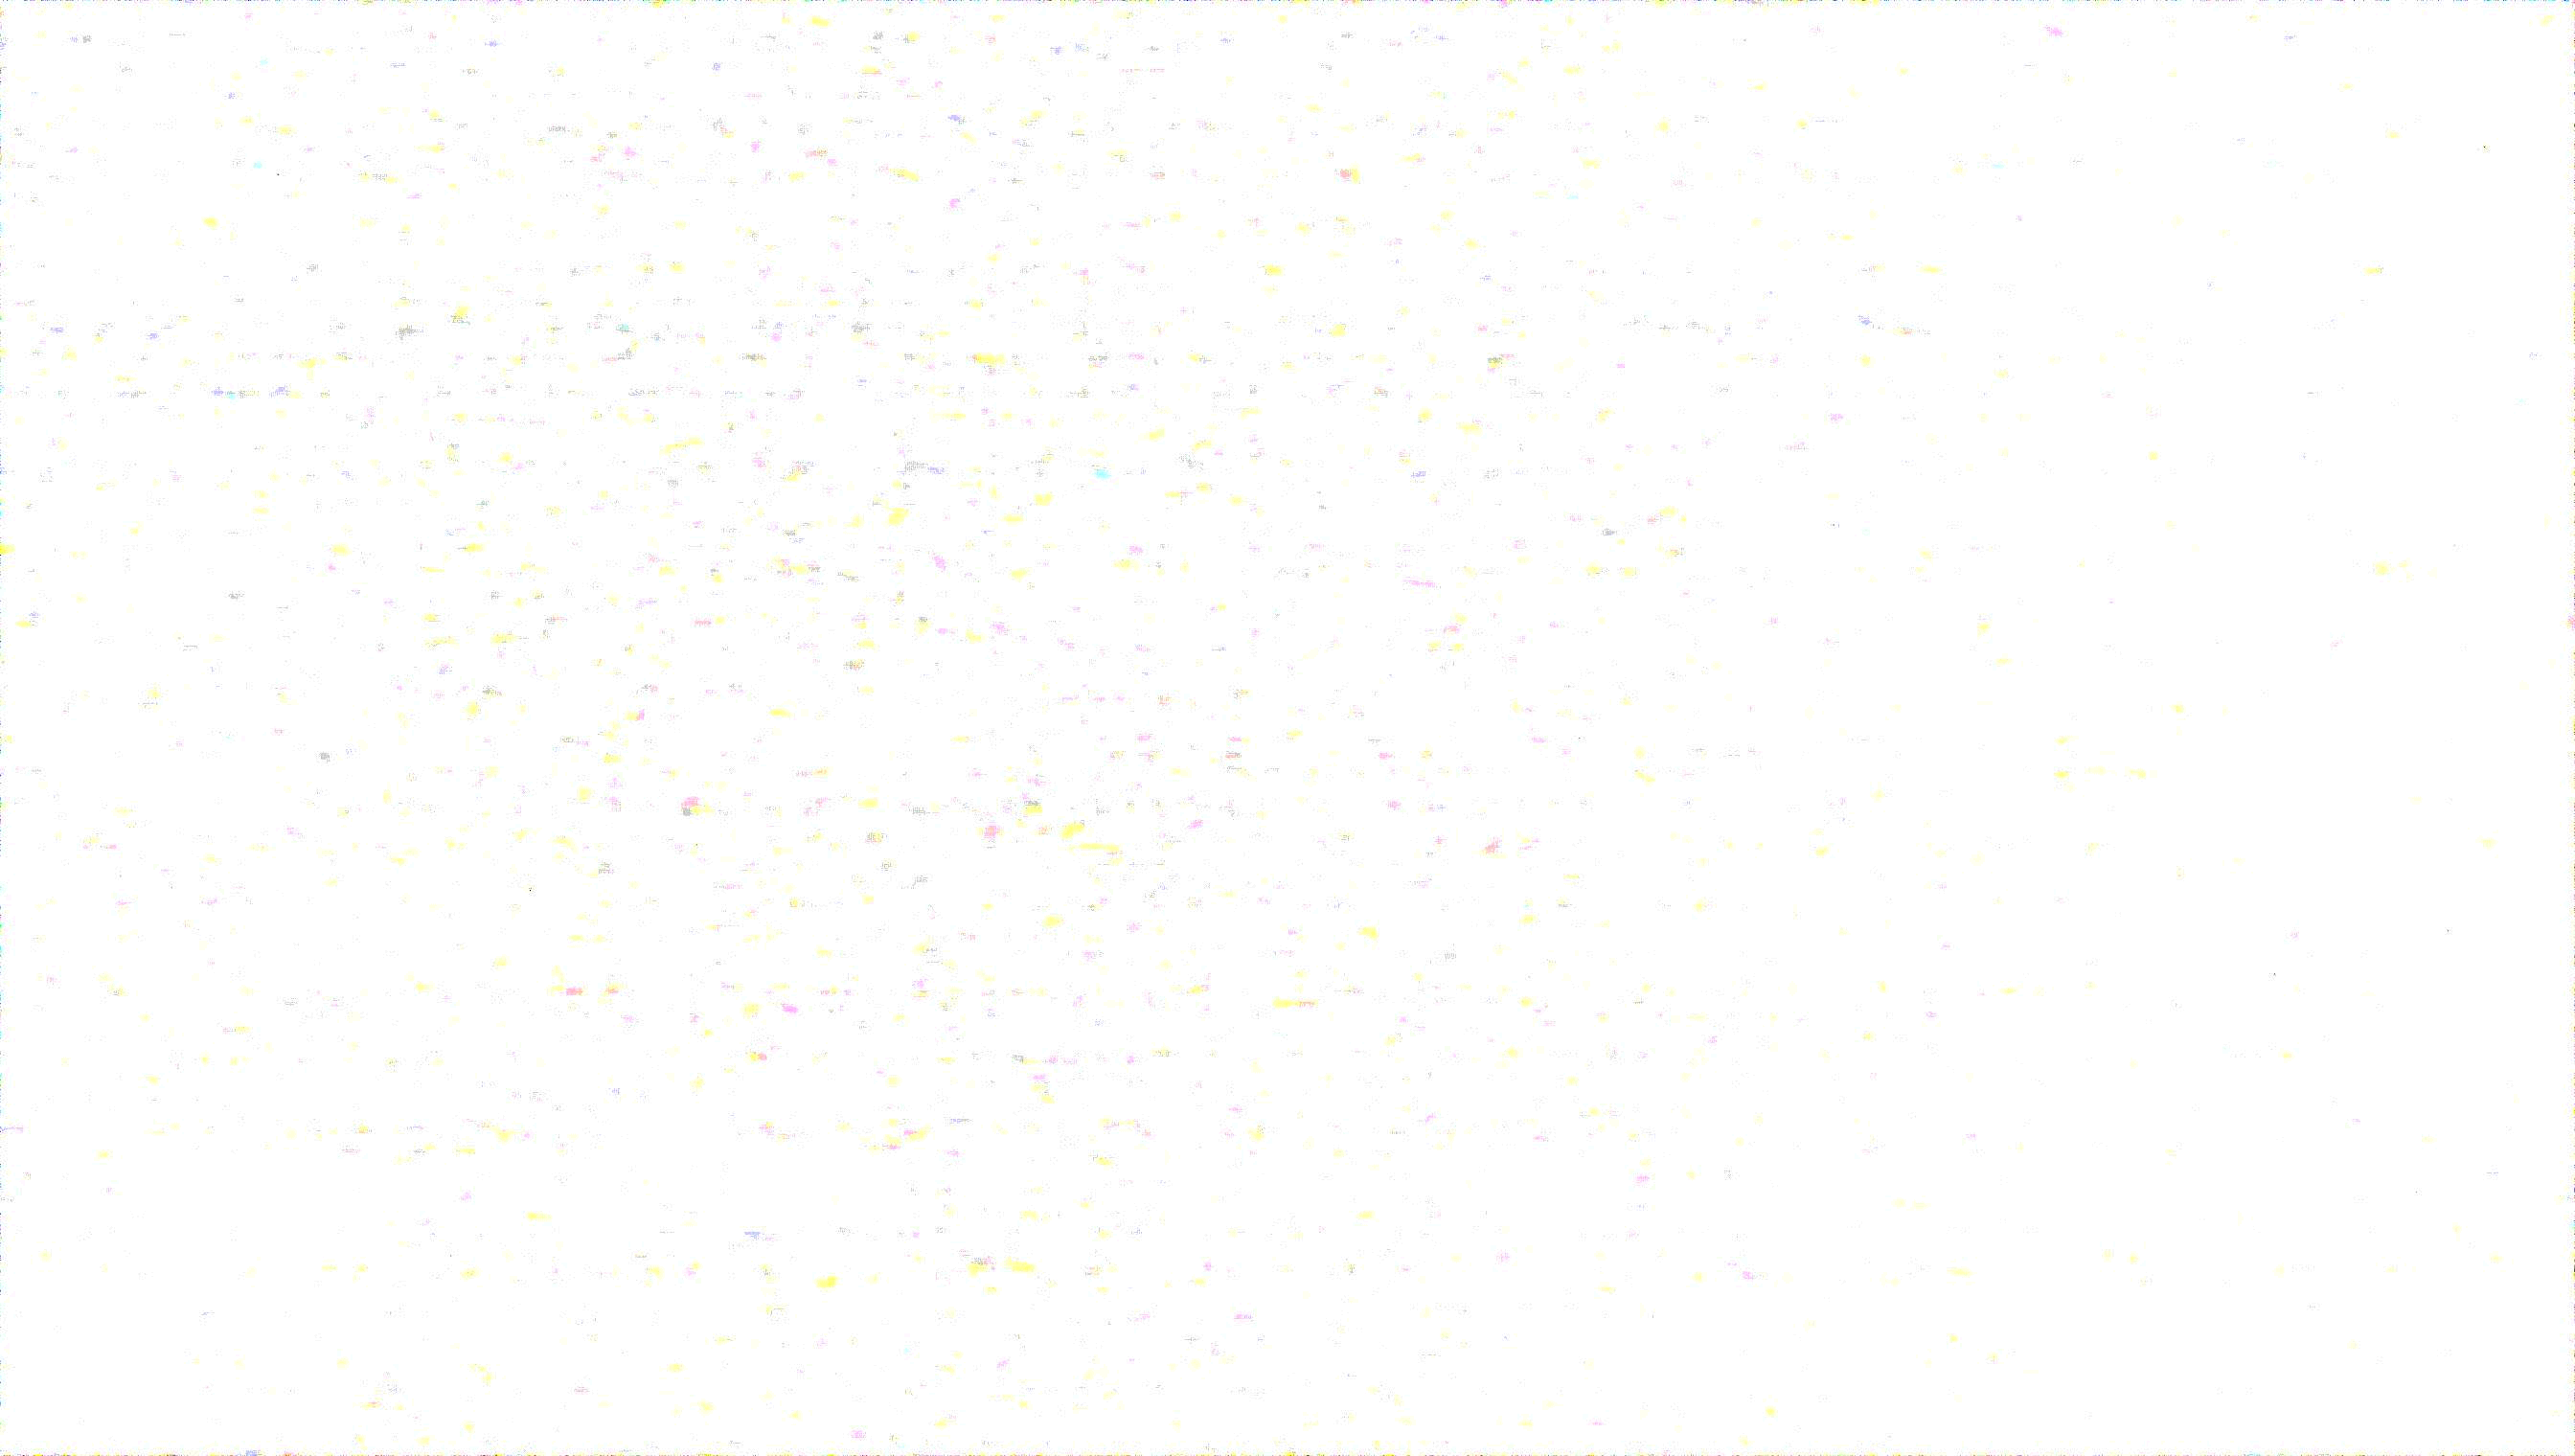
\includegraphics[width=1\linewidth]{img/NoisHight}}
%	\caption{Aufnahme eines Schwarz-Bildes $(2688\times 1520)$ der Actioncam um den Faktor 7 verstärkt und invertiert.}
%	\label{img_noishight}
%\end{figure}
Für die Umsetzung wurden Open Source Computer Vision (OpenCV 3.1) verwendet. Dies ist eine C/C++ Bibliothek von Algorithmen zur Bildverarbeitung in Echtzeit, veröffentlicht unter der BSD Lizenz (Berkeley
Software Distribution)\\
\cite{OpenCv_What_Is}\cite{wiki_Wha_is_OPenCV}
\section{Software}
Für die Umsetzung werden folgende Software-Elemente aus fremder Quelle verwendet.
\subsection{ElSe}
Ellipse Selection for Robust Pupil Detection in Real-World Environments, ein Algorithmus zur Bestimmung der Pupille in einem Bild. Der Ursprüngliche ElSe-Algorithmus ist für Graubilder mit Infrarotbeleuchtung ausgelegt, wurde für diese Anwendung angepasst um Farbbilder verarbeiten zu können.\\
Entwickelt von der Uni Tübingen. \cite{ElSe}
\subsection{MTCNN Face Detection}
Multi-task Cascaded Convolutional Networks, ein Algorithmus zur Detektion von Gesichtern und Bestimmung von 5 Gesichts-Landmarks in Farbbilder. Dabei werden drei CNN auf einer Bildpyramide angewendet um so zuverlässig Gesichter mit verschiedenster Größe zu erkennen.\\
\cite{MTCCN}
\subsection{OpenCV}
Open Source Computer Vision, ist eine C/C++ Bibliothek von Algorithmen zur Bildverarbeitung in Echtzeit unter der BSD Lizenz (Berkeley
Software Distribution)\\
\cite{wiki_Wha_is_OPenCV}\cite{OpenCv_What_Is}
\subsection{OpenFace}
Ein Open-Source Echtzeitverfahren auf Basis von CLNF zur Bestimmung und Analyse von Gesichtsmerkmalen in Grau-Bildern und Videos. Dabei werden 68 signifikante Punkte im Gesicht bestimmt und auf Basis jener Position und Orientierung ermittelt.\\
Entwickelt von der University of Cambridge \cite{OpenFace}


\chapter{Theorie \& Grundlage}
\section{Grundlagen}
Gesichtserkennung ist eine der fortschrittlichen Verfahren in der maschinellen Bildverarbeitung und wird ständig weiter entwickelt. Darunter fallen neben der Detektion des Gesichtes auch seine Analyse wie Orientierung oder das Erkennen von Mimik wie Lächeln bei Kameras und Übereinstimmungen.\\
Bei vielen Anwendungen ist der Stand der Technik oft ein Neuronales Netz beteiligt.
\subsection{Künstliches neuronales Netz}
Ein künstliches neuronales Netz besteht aus miteinander verknüpften künstlichen Neuronen. Jedes Neuron erhält Eingangswerte und besitzt einen Ausgabewert.\\
Um die Ausgabe zu bestimmen, werden die einzelne Eingangswerte des Neurons individuell Gewichtet, mittels einer Übertragungsfunktion zusammengefasst und durch eine Schwellenwertfunktion das Ergebnis bestimmt.\\
Um die Parameter (Gewichtung und Funktionen) des Neurons zu bestimmen, wird es zufällig initialisiert und dann so angepasst, dass es zu einer gegebenen Eingabe das Gewünschte Ergebnis liefert und der Fehler über dem gesamten Trainingsdatensatzes minimal ist.\\
Soll ein gesamtes Netz trainiert werden, so wird jedes einzelne Neuron zufällig Initialisiert und anschließend so angepasst das der Fehler auf einem Trainingsdatensatz minimal ist.\\
\cite{Maschin_Neuron}
\subsection{Convolutional Neural Network (CNN)}
CNN ist eine Weiterentwicklung der neuronalen Netze die vor allem im Bereich Klassifizierung eingesetzt werden, unter anderem bei der Bild- und Spracherkennung. Der unterschied liegt bei der Verwendung von gewichteten Faltungen der Eingabe erreicht. Die CNN definieren in vielen Anwendungsbereichen momentan der Stand der Technik.\\
Durch die Faltung werden die Information aus den umliegenden Punkten eines Bereiches zusammengefasst und komprimiert an die nächste Schicht weitergegeben, um in der untersten Schicht alle vorhanden Informationen zusammenzuführen. 
Der Faltungskern kann je nach Anwendung beliebig gestaltet sein, so ist eine Glättung durch einen Gauß-Kernel oder Kantendetektion durch einen Kirsch-Operator möglich.\\
Ein CNN kann in zwei Bereiche aufgeteilt werden, Feature Extraktion und Klassifizierung. Bei der Feature Extraktion werden verschiedene Kernel und Komprimierung auf den Eingabeinformationen angewendet um sie für den zweiten Teil aufzubereiten.
Gelernt werden können jeder einzelne Kernel für sich und die jeweiligen Bewertungen der einzelnen Kernel und Neuronen.\\
Quelle \& Bild
\subsection{Constrained Local Model (CLM)}
Dies ist ein Verfahren um mehrere Punkte eines Objektes zu lokalisieren. Dabei wird eine Wahrscheinlichkeitskarte für jeden einzelnen Punkt erstellt, wo dieser sich aufhalten kann, auf Basis eines Trainingsdatensatzes. Nun wird versucht für das Bild, auf welchem gerechnet werden soll, für jeden Punkt den maximalen Wert zu erreichen zwischen passendem Farbverlauf und seiner Wahrscheinlichkeit.\\
Dieser Art der Bestimmung von Punkten mit Positionsabhängigkeiten ist ziemlich zuverlässig und dennoch dynamisch genug um auch mit kleinen Veränderungen klar zu kommen.\\
Dies ist Wichtig, bei der Detektion von leicht verformbaren Objekten wie Gesichter und ist zuverlässiger als das Active Appearance Model (AAM).\\
Quelle \& Detecton der Landmarks
\subsection{Active Appearance Model (AAM)}
Dies ist ein Verfahren der Bildverarbeitung um Übereinstimmungen zu einem Modell zu finden. Dazu wird aus dem Trainingsdatensatz eine typische einheitliche Form des Objektes generiert mit seinen signifikanten Landmarks.\\
Soll nun zu eine Eingabebild die Übereinstimmung ermittelt werden, wird zuerst versucht es bestmöglich mittels Transformation in die typische einheitliche Form zu überführen. Sind dennoch Unterschiede vorhanden, liegt diese an der Erscheinung des Objektes.\\
\cite{wiki_AAM}
\subsection{Point Distribution Model (PDM) \& Generalized Adaptive View-based Appearance Model (GAVAM)}
Mit Point Distribution Model (PDM) können verformbare Objekte recht gut modelliert werden. Dabei wird die durchschnittliche Form $\overline{X}$ des Objekts anhand der Eingabe bestimmt und eine Matrix $P$ von Eigenvektoren ermittelt, um die möglichen Deformierungen darzustellen.
\begin{align*}
X &= \overline{X}+P\cdot b
\end{align*}
Somit kann durch einen Skalierungsvektor $b$ alle möglichen der Eingabeformen $X$ des Objektes aus dem Durchschnittsmodell dargestellt werden. Zur Vereinfachung reicht es, die signifikantesten Eigenvektoren in $P$ auf zu nehmen und dennoch $X$ ausreichend genau beschreiben zu können.\\
Ist bekannt welche Art der Verformung durch den Eingenvektor dargestellt ist, z.B. eine bestimmte Orientierung, so kann anhand des Skallierungsvektors die Rotation der Eingabe bestimmt werden, siehe Generalized Adaptive View-based Appearance Model (GAVAM).\\
Eine Problematik bei dieser Art der Bestimmung der Rotation entsteht, wenn neben der Verschiebung der Landmarks durch die Rotation, auch eine Deformierung des Objektes stattgefunden hat und somit keine eindeutige Lösung gefunden werden kann. Dies ist eine Problematik, wenn auf Gesichtern gerechnet wird, da immer eine Veränderung der Mundwinkel oder Augenlider vorhanden ist.\\
\cite{wiki_PDM}\cite{pdf_PDM}\cite{pdf_GAVAM}
\subsection{Non-maximum suppression  (NMS)}
Ein Verfahren um Kanten in einem Bild exakter zu bestimmen. Dabei wird der Farbwert des Pixels mit dem umliegenden verglichen und sollte es nicht maximal sein auf Null gesetzt.\\
Auf diese Weise bleibt nur noch ein Kantenpixel übrig. 
\section{MTCNN Face Detection}
\label{MTCNN}
Bei Multi-task Cascaded Convolutional Network handelt es sich um ein Verfahren dass bei der Detektion von Gesichtern auch deren Ausrichtung berücksichtigt wird, um so bessere Ergebnis zu erzielen.
\subsection{Anforderungen}
Sein Einsatzgebiet ist die Vorverarbeitung eines Frames für die spätere Auswertung. Somit soll dieser Schritt von einem möglichst robusten Verfahren zur Detektion von Gesichtern durchgeführt werden.\\
Dabei wird auf recht großen Bild gearbeitet mit verhältnismäßig kleinen und verschieden großen Gesichtern.\\
Außerdem sollte das Verfahren ausreichend schnell sein, da es sich hierbei nur um ein Vorverarbeitungsschritt handelt und zur Beschleunigung der späteren Berechnung beitragen soll.
\subsection{Die 3 Stufen der Verarbeitung}
Für die gute Detektionsqualität sorgt die dreistufige Verarbeitung auf der Bildpyramide. Bei der Bildpyramide handelt es ich um ein in verschiedenen Größen skaliertes Bild, damit der Gesuchte Inhalt in der gewünschten Auflösung abgebildet ist, ohne dass etwas über den Inhalt bekannt ist.\\
Dies ist von Vorteil, damit das CNN auf eine feste Größe von Gesichtern optimiert werden kann, um neben dem möglichen Farbverläufen, durch die Skalierung das Lernen nicht zusätzlich zu erschweren.
\begin{figure}
	\centering
	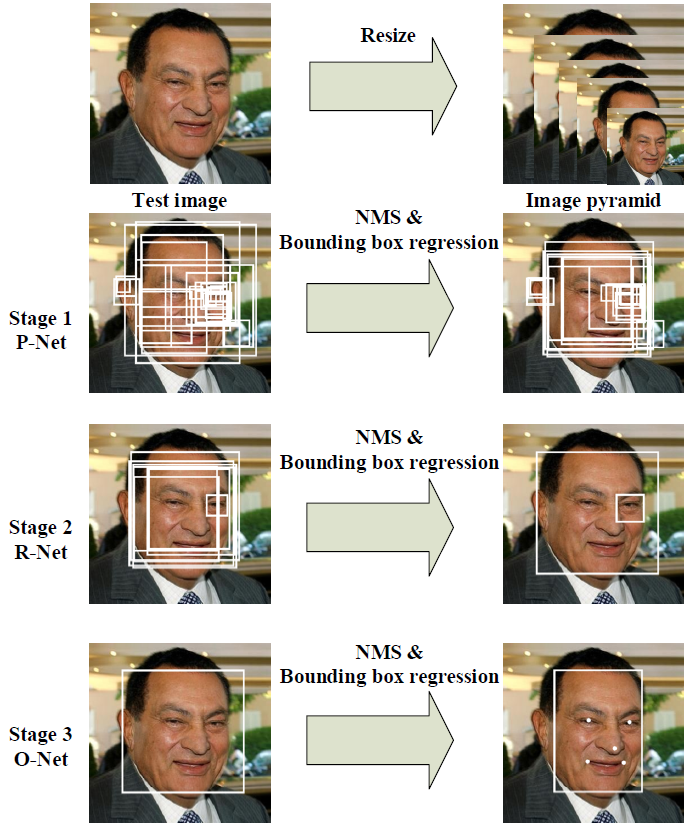
\includegraphics[width=0.5\linewidth]{img/MTCNN_Step}
	\caption{Darstellung des Funktionsablaufes von MTCCN\cite{MTCCN}}
	\label{img_MTCNN_Step}
\end{figure}
\subsubsection{Stufe 1}
Beim ersten Verarbeitungsschritt erden alle Bereiche eines Bilds gesucht, in denen möglicherweise ein Gesicht zu sehen ist. Dazu wird zuerst ein einfaches CNN eingesetzt und die Ergebnisse, die sich sehr stark überlappen, zusammengefasst.\\
Für die Detektion wird von einem CNN, dem sogenannte Proposal Network (P-Net), eingesetzt und sehr viele Bounding-Boxen ermittelt. Diese werden nun mit einem NMS ausgedünnt, um die am stärksten überlappenden Bounding-Boxen zusammen zu fassen.
\subsubsection{Stufe 2}
Anschließend werden die möglichen Bereiche mittels eines weiten CNN analysiert, damit alle Nicht-Gesichtsbereiche erkannt und entfernt werden können.\\
Dies wird von dem Refine Network (R-Net) übernommen und anschließend die möglichen Bounding-Boxen mittels NMS weiter reduziert.
\subsubsection{Stufe 3}
Der letzte Schritt wird von einem deutlich genaueren CNN übernommen, um ein Gesicht zu detektieren, dem sogenannten Output Network (O-Net). Womit die resultierenden exakten Boxen und 5 Landmarks ermittelt werden.
\subsection{Qualität}
MTCNN Face Detection ist bei der Zuverlässigkeit im Verglich zu anderen bekannten Verfahren überlegen, siehe \autoref{img_MTCNN_quality} und zudem Echtzeit fähig. Im Test-Datensatz sind auch Gesichtern mit einer Größe von $20\times 20$ enthalten und wurden erfolgreich erkannt.\\
Somit sind alle Anforderungen erfüllt um mit diesem Verfahren den vorhanden Frame für die nachfolgenden Berechnungen vorzubereiten, daher wird es auch hier eingesetzt.
\begin{figure}
	\centering
	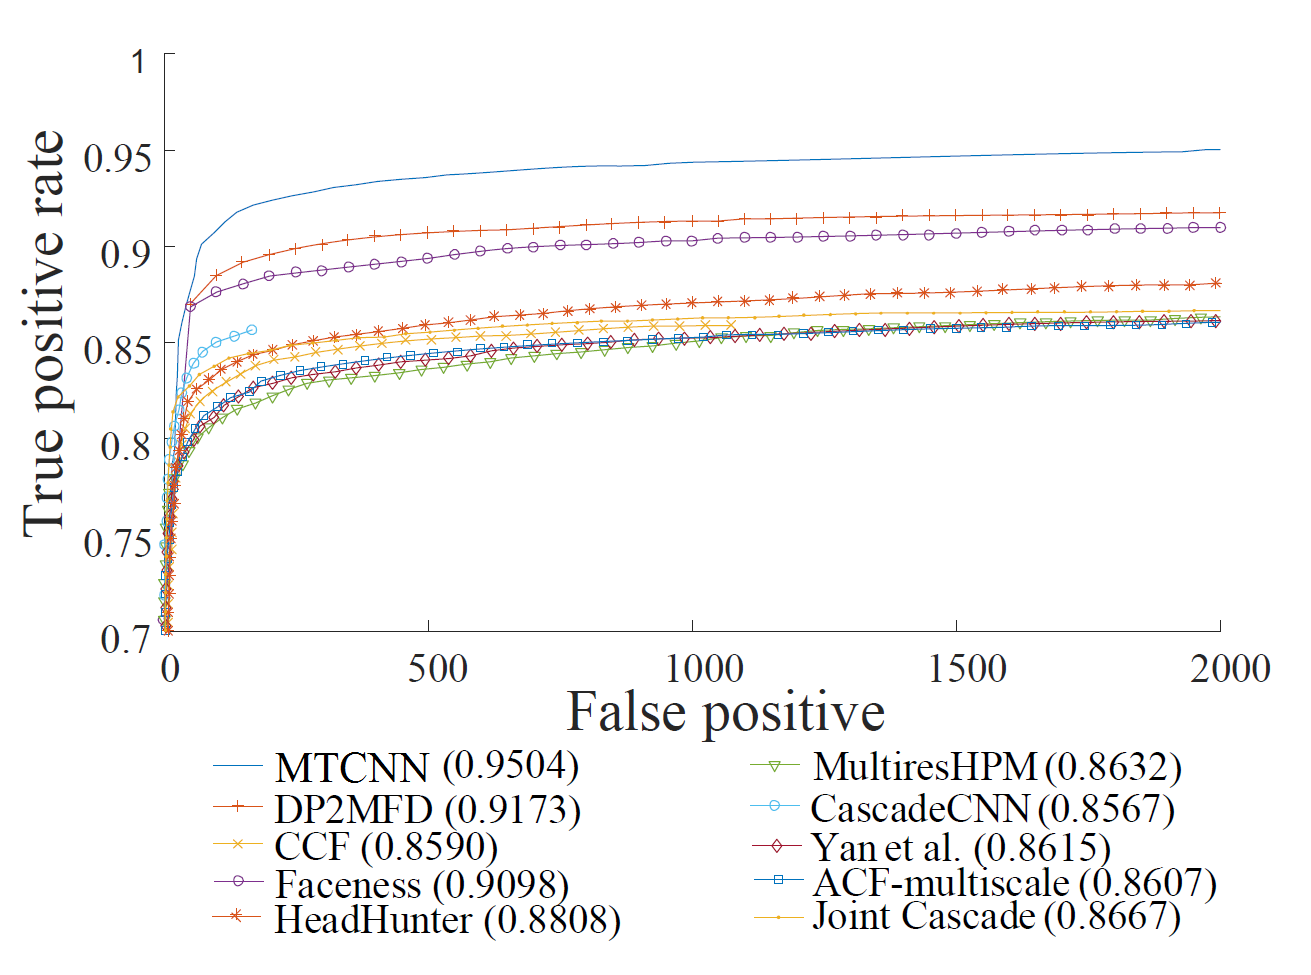
\includegraphics[width=0.5\linewidth]{img/MTCNN_quality}
	\caption{normale blaue Linie\cite{MTCCN}}
	\label{img_MTCNN_quality}
\end{figure}
%Joint Face Detection and Alignment using Multi-task Cascaded Convolutional Networks
\subsection{Skalieren von Bildern}
Da die Berechnungen meist auf recht kleinen Bildausschnitten ausgeführt werden muss, müssen diese für die weiteren Rechenschritte Hochskaliert werden.\\
Dabei ist es wichtig, dass die Gesichtsmerkmale möglichst gut rekonstruiert werden damit die entsprechenden Landmarks gefunden und bestimmt werden können.
\subsubsection{Nearest-Neighbor}
Verwende gleicher Farbwert wie das Nächstgelegene Pixel. Dadurch werden nur die ehemaligen Pixel größer und das Gesicht wirkt sehr Kantig.\\
To Do! - Bsp Bilder
\subsubsection{Linear}
Dabei wird zwischen den umliegenden nächst gelegenen Pixel Interpoliert, wodurch weitere Farbwerte entstehen und das Ergebnis gleichmäßiger aber unscharf wirkt.
To Do! - Bsp Bilder
\subsubsection{Bicubic}
Um den Farbwert zu ermitteln, werden die umliegenden $4\times 4$ Pixelwerte betrachtet um den Farbverlauf als eine Funktion 3. Grades zu bestimmen. Somit werden feinere Details besser dargestellt als beim Linearen verfahren, allerdings kann es durch den bestimmten Verlauf auch zum Überschwingen kommen, wodurch Fehlfarben entstehen können.\\
To Do! - Bsp Bilder
%%https://en.wikipedia.org/wiki/Bicubic_interpolation
\subsubsection{Lanczos}
Dieser Filter besteht aus einer Sinc-Funktion über einen Bereich, um so eine Bewertung der Benachbarten Pixelwerte zu erhalten. Somit kann ergibt sich der Neue Farbwert aus den bewerteten umliegenden Pixeln.\\
To Do! - Bsp Bilder
%%To Do! - Bsp Bilder

%% http://docs.opencv.org/2.4/modules/imgproc/doc/geometric_transformations.html#resize
\section{OpenFace}
Die Aufgaben von OpenFace ist die Analyse der Gesichtes aus Bildern. Dabei sind nur die Kameraparameter bekannt und keinerlei Zusätze wie eine Tiefenbild oder Infrarotbeleuchtung der Szene. Dabei ist für die Anwendung die Kopfposition (Translation und Orientierung) und Blickrichtung von Interesse, da mit ihnen zurückrechnet werden kann wohin der Schüler schaut.\\
OpenFace kann neben den Landmarks auch die Position, Blickrichtung und Gesichtsmerkmale bestimmen, basierend auf einem einfachen Bild. Sollte ein Video als Quelle fungieren, so kann OpenFace auch lernen. 
\subsection{Verarbeitungsschritte}
Der Rechenaufwand ist so ausgelegt, dass alle Berechnungen auf einer Webcam in Echtzeit ausgeführt werden können, dies ist im aktuellen Fall nicht notwendig, da es sich um eine nachträgliche Auswertung handelt. Durch den Aufbau sind nur recht kleine Farbbilder der Gesichter in einem Video vorhanden wodurch eine Auswertung erschwert wird.
\subsubsection{Gesichts-Landmarks: Detektion und Verfolgung}
Für die Bestimmung und Tracking der Landmarks wird ein Conditional Local Neural Fields (CLNF) eingesetzt. Dabei Handels es sich im Grunde um ein Constrained Local Model (CLM) nur mit verbesserter Patch Experts und Optimierungsfunktionen.\\
Zu Beginn werden verschiedene initiale Hypothesen aus dlib-Bibliothek verwendet und die Passende ausgewählt. Bei den initiale Hypothesen handelt es sich um verschiedene Gesichtsorientierungen auf denen verschiedene Netze gelernt wurden. Dies ist zwar langsamer, aber auch exakter als eine einfache Hypothese.\\
Wird ein Tracing auf Videos gemacht, so wird als initiale Hypothese das Ergebnis aus dem letzten Frame verwendet.\\
Sollte das Tracing scheitern, so wird das CNN reseted um Neu zu beginnen.
Die beiden Hauptkomponenten ist das Point Distribution Model (PDM) zur Erfassung der Anordnung der Landmarks und patch experts zum Erfassen der Variante der einzelnen Landmarks.\\
Auf diese weise werden 68 Gesichts-Landmarks und  weitere 28 pro Auge erfasst. Zur Brechung auf den Gesichtern sollte es eine Mindestbreite von 100 Pixeln für eine zuverlässige Detektion Originalgröße besitzt.
\subsubsection{Bestimmung der Gesichtsposition}
Zur Bestimmung der Translation und Orientierung des Gesichtes wird ein CLNF eingesetzt. Dabei wurde es mit der Kameraabbildung der 3D-Landmarks eines Kopfes in verschiedenen Positionen initialisiert. Womit auf eine Normierte Abbildung berechnet wird, diese kann mit den passenden Kameraparameter für die Aufnahme angepasst werden um die reale Position zu bestimmen. Sind keine bekannt, so können diese geschätzt werden.\\
Bei der Schätzung der Brennweite für ein Bild mit einer Dimension $I_x\times I_y$ wird das Standardobjektiv mit 50 mm und einer Auflösung von $640 \times 480$ Pixel angenommen, somit ergibt sich für die Brennweiten $f_x$ und $f_y$:
\begin{align*}
f_x = 500\cdot \frac{I_x}{640}\\
f_y = 500\cdot \frac{I_y}{480}
\end{align*}
\subsubsection{Bestimmung der Blickrichtung}
Durch die Landmarks der Augen werden die Augenlider, Iris und Pupille dargestellt und für jedes Auge separat bestimmt. Dabei wird der Augenbereich, basierend auf dem Gesicht, verwendet um mit einem weiten CNN die 28 Landmarks zu bestimmen.\\
Zur Bestimmung der Blickrichtung wird wie folgt vorgegeben. Zuerst wird der Strahl bestimmt der, ausgehend vom Zentrum der Kamera, durch das Zentrum der Pupille verläuft. Nun wir der Schnittpunkt zwischen diesem Strahl und einer Sphäre bestimmt, die das Auge repräsentiert. Nun wird ein Strahl bestimmt der vom Zentrum der Sphäre ausgehend durch den berechneten Schnittpunkt verläuft, dies ist die resultierende Blickrichtung.
\subsubsection{Detection der Gesichtsmerkmale}
Dieser Schritt kann von OpenFace ausgeführt werden, ist aber  im aktuellen Fall nicht von Relevanz.
\subsection{Veröffentlichte Genauigkeit}
Die Messung wurde auf de Biwi Kinect head pose dataset und BU dataset. Für die Genauigkeit der Kopfposition haben sich folgend Werte ergeben in Grad:\\
\begin{tabular}{|l|c|c|c||c|c|}
	\hline
	&Yaw&Pitch&Roll&Mean&Median\\\hline
	Biwi Kinect \cite{BIWI_database}&7.9&5.6&4.5&6.0&2.6\\\hline
	BU dataset \cite{BU_database}&2.8&3.3&2.3&2.8&2.0\\\hline
	ICT-3DHP \cite{ICT_database} &3.6&3.6&3.6&3.6&-\\\hline
\end{tabular}\\\\
Für die Qualität zur Bestimmung der Blickrichtung ergab sich ein durchschnittlichen Fehler von 9.96 Grad.
\section{Augenanalyse mit Ellipse Selection for Robust Pupil Detection (ElSe)}
\label{ElSe}
Zur Bestimmung der Blickrichtung ist die Augenregion natürlich von besonderer Bedeutung. Aus diesem Grund werden die Landmarks der Augenregion nochmals gesondert betrachtet. Aufgrund der besonderen Bedeutung existiert eine große Anzahl an Algorithmen, die speziell auf eine hochgenaue Bestimmung von Augenmerkmalen optimiert sind, wie beispielsweise ElSe \cite{ElSe}, Goutam \cite{Eye_FastCorner}, Starburst \cite{Starburst} oder Swirski \cite{Swirski2012}. Auch OpenFace verwendet ein zusätzlich dafür trainiertes CLNF, um weiter 28 LAndmarks pro Auge zu bestimmen, zusätzlich zu den 64 Landmarks das Gesicht. Aus diesen Augen-Landmarks, die Lider, Iris und Pupille dargestellen kann die Blickrichtung ermittelt werden.\\
Um die Position der Landmarks zu verbessern, kann auf den Augenbereichen der ElSe-Algotithmus eingesetzt werden. Dieser Algorithmus basiert auf einem rechnerischen Ansatz und nicht auf Neuronen um die Umrisse der Pupille zu berechnen. Für die Verbesserung wurde das ElSe-Verfahren wurde gewählt, da es im Test \cite{ElSe} am besten abgeschnitten hat und direkt das Zentrum der Pupille liefert.\\
Der ursprüngliche ElSe-Algorithmus ist für Graubilder einer Eye-Tracking-Brille ausgelegt und optimiert, zudem ist es auf diesen Bildern zu einer Echtzeitauswertung in der Lage. Dieser Anwendungsbereich betrifft vor allem die Anforderung an eine hohe Qualität der Aufnahme im Bezug auf die Auflösung und der Infrarotbeleuchtung des Bildes. Die Infrarotbeleuchtung wird verwendet, damit das Auge ausreichend beleuchtet ist ohne den Probanden zu blenden. Diese Voraussetzungen führen dazu, das die Detektionsleistung bei niedriger auflösenden Bildern rasch abnimmt.\\
Als Ergebnis liefert ElSe eine Ellipse, die den Umriss der Pupille im Bild beschreibt. Aus dieser Ellipse können die Landmarks der Pupille abgeleitet werden.\\
Für den Test im Paper wurden Bilder von $384\times 288$ Pixel Größe verwendet und im Vergleich zu den anderen Verfahren ist ElSe in den meisten Fällen überlegen, mit einer Verbesserung der Erkennungsrate um $14.53\%$ auf dem verwendeten Datensatz.\cite{ElSe}\\
Für die Anwendung wurde der ursprüngliche ElSe-Algorithmus angepasst, um auf Farbbildern die nach Grau konvertiert wurden arbeiten zu können.
\subsection{Pupille bestimmen mit Kantendetektion}
Da die Pupille als schwarzen Fleck im Bild dargestellt ist und die Iris einen helleren Farbton aufweist, wird ein Kantendetektor verwendet, der alle Pixel markiert, bei denen eine starke Farbänderung auftritt. Bei ElSe wird ein morphologischen Ansatz eingesetzt, von Relevanz sind nur zusammenhängende Kantenpixel um die Kante zwischen Pupille und Iris zu finden. Alle anderen Pixel können ignoriert werden, wobei jedes Kantenpixel als Startpunkt der Berechnung dienen kann.\\
Um jene Kantenpixel zu erhalten, die die Pupille beschreiben, wird versucht fortlaufende Kanten zu finden, die eine Ellipse bilden. Jene die nicht diesen Anforderungen entsprechen, können recht schnell ignoriert werden. Anschließend werden auch alle offenen Ellipsenverläufe und jene Kantenpixel die am meisten vom bestimmten Verlauf abweichen, verworfen.\\
Das beste Ergebnis aller bestimmten Ellipsen wird als Lösung verwendet.
\subsection{Grobe Bestimmung der Pupille}
\label{ElSe_Grob}
Sollte die Bestimmung der Ellipse, wie im vorigen Kapitel beschreiben, scheitern, so wird das Zentrum des dunkelsten Kreises ermittelt. So ein Punkt kann immer gefunden werden, ist aber nicht zwingend die Pupille.\\
Auf einem verkleinerten Bild, \autoref{img_else} (1), wird ein kreisförmiger Mean-Filter eingesetzt mit Ergebnis in \autoref{img_else} (3). Zur zweiten Faltung wird der Durchschnitt über ein Quadrat ohne inneren Kreis eingesetzt mit Ergebnis in \autoref{img_else} (2), wobei für beide Kreisen der selbe Radius verwendet wird.\\
Nun wird das Ergebnis des Quadratischen Mean-Filters invertiert, \autoref{img_else} (4), und mittels Punkt-Multiplikation mit dem anderen Meanfilter zusammengebracht, \autoref{img_else} (5). Im resultierendem Bild wird nun der höchste Wert gesucht, da dies das Zentrum des dunkelsten kreisförmigen Ortes im Bild ist.\\
Ergebnis des Beispiels ist als Kreuz in \autoref{img_else} (6) markiert. 
\begin{figure}
	\centering
	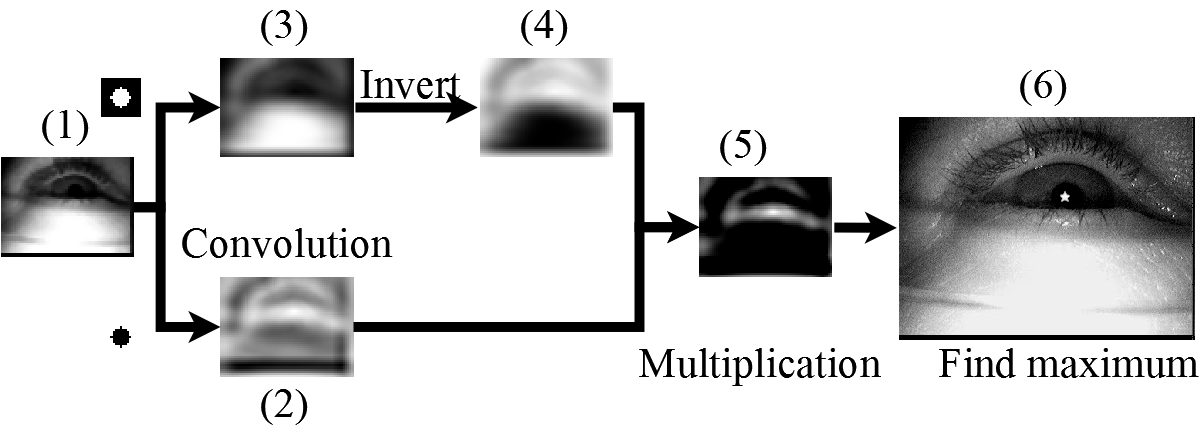
\includegraphics[width=0.8\linewidth]{img/ElSe}
	\caption{Ablauf der alternativen Berechnung zur Pupillen-Detektion von \cite{ElSe}}
	\label{img_else}
\end{figure}
\section{Berechnung der Position}
\label{calc_Position}
Zur Bestimmung der Position $P=(X_{avg};Y_{avg};Z_{avg})$ des Gesichtes im Kamerakoordinaten wird die Größe, ein Skalierungsfaktor $S$, des Kopfes im Bild verwendet.\\
Da bei der Abbildung von den Koordinaten ins Bild gilt $x=f\cdot \frac{X}{Z}$ und $ y=f\cdot \frac{Y}{Z}$, somit kann die Tiefe wie folgt abgeschätzt werden.\\
Sei $P_1 = (X_1;Y_1;Z_1), P_2=(X_2;Y_2;Z_2)$ die Beschreibung der Größe $G$ eines Kopfes mit:\\
\begin{align*}
a &= \frac{\sqrt{(X_1-X_2)^2+(Y_1+Y_2)^2}}{\frac{Z_1-Z_2}{2}} =\frac{G}{Z_{avg}}\\
S &= \frac{S_G}{G}\\
\Rightarrow a\cdot f &= f\cdot\frac{G}{Z_{avg}} = S_G\\
Z_{avg} &= \frac{f}{S_G}\cdot G = \frac{f}{S}\\
X_{avg} &= \frac{x \cdot Z_{avg}}{f}\\
Y_{avg} &= \frac{y \cdot Z_{avg}}{f}\\
\end{align*}
Dies beschreibt allerdings nur eine Annäherung an die Tatsächliche Position, da mit einem Durchschnittlichen Kopfgröße gerechnet wird.
\subsection{Zusammenhang Bildposition \& Weltposition}
Als Ausgangspunkt werden die Ergebnisse des CNN eingesetzt um mit deren Hilfe wie in \autoref{calc_Position} beschreiben die Position zu bestimmen. Zur Bestimmung der Orientierung $R$ liefert auch das CNN ein Ergebnis $R_{CNN}$. Allerdings stimmt es nur im Zentrum des Bildes, da am Rand immer mehr die Orientierung der einzelnen Pixel mit berücksichtigt werden muss.\\
\begin{align*}
euler_x &= \tan^{-1}(\frac{\sqrt{X^2+Z^2}}{Z^2})\\
euler_y &= \tan^{-1}(\frac{\sqrt{Y^2+Z^2}}{Z^2})\\
R_{pos} &= R(euler_x,euler_y,0)\\
R &= R_{CNN}\cdot R{pos}
\end{align*}
Eine weitere Verbesserung kann erreicht werden, indem die gefunden 2D-Landmarks mit Hilfe des PDM in 3D zu überführen. Um anschließend die Überführung von 2D nach 3D-Koordinaten erneut zu bestimmen um die Orientierung und Position zu ermitteln. Auch bei diesem Verfahren muss die Pixelorientierung beachtete werden.

\chapter{Implementierung}
\section{Ablauf der Implementierung}
\subsection{Umsetzung Graph}
\begin{frame}
\begin{center}
\begin{footnotesize}
\begin{tikzpicture}
	\node[circle,draw,align=center] (C) at(0,0) {Kamera};
	\node[draw,align=center] (F) at(0,-2)  {Gesichtserkennung};
	\node[draw,align=center] (S) at(0,-3.1)  {Skalierung};
	\node[draw,align=center] (G) at(6,-4.2)  {Graukonvertierung};
	\node[draw,align=center] (A) at(0,-4.2)  {Gesichtsanalyse};
	\node[draw,align=center] (E) at(6,-5.3)  {Augenanalyse};
	
	\node (outA) at(0,-7.3)  {};
	\node (outB) at(6,-7.3)  {};
	
	\draw[->] (E)to node[right,align=center]{Blickrichtung}(outB);
	\draw[->] (A)to[out=-45,in=90] node[right]{}(outB);
	
	\draw[->] (C)to node[right]{Frame}(F);
	\draw[->] (F)to node[right]{Bildausschnitt}(S);
	\draw[->] (S)to node[right]{Eingabebild}(A);
	\draw[->] (A)to node[left,align=center]{Gesichts-\\orientierung}(outA);
	
	\draw[->] (A)to node[below]{Augenbereich}(G);
	\draw[->] (C)to[out=-45,in=90] node[left]{}(G);
	\draw[->] (G)to node[right]{Eingabebild}(E);
\end{tikzpicture}
\end{footnotesize}
\end{center}
\end{frame}
Zur Bestimmung der Blickrichtung sowie Kopfposition und Orientierung wird ein mehrstufiges Verfahren eingesetzt:\\
Zuerst müssen alle Gesichter, die im aktuellen Videobild vorhanden sind, detektiert werden, siehe \autoref{MTCNN}. Dabei machen die relevanten Bereiche nur einen sehr geringen Anteil des gesamten Bildes aus.\\
Da Gesichtserkennung und Landmark Erkennung auf unterschiedlichen großen Gesichtsbereichen arbeiten (z.B. Haare und Kinn teilweise als Gesicht zählen, teilweise nicht) ist ein Zwischenschritt zur Vergrößerung der erkannten Bereiche notwendig, damit das gesamte Gesicht abgebildet ist.\\
Ist ein Gesicht in mehreren Einzelnbildern des Videos abgebildet, so muss auch eine Identitätszuordnung vorgenommen werden, damit dem Computerprogramm bekannt ist welches Gesicht in Bild 1 welchem in Bild 2 entspricht. Für die Zuordnung reicht es meist aus, jene Box zu wählen, die am ehesten den selben Bildausschnitt repräsentiert entweder über ähnliche Positionierung im Videobild oder über die Bildähnlichkeit da ein Kopf zwischen zwei schnell aufeinanderfolgenden Einzelbildern nur limitiert bewegen kann.\\
Damit sicher auf allen Gesichtern gerechnet werden kann, ist eine semiautomatische Korrektur erforderlich um Falsch-Detektionen zu entfernen und fehlende Boxen der Gesichter ergänzen zu können. Daher können alle bisher unternommenen Schritte auch von anderen Verfahren übernommen werden, da es sich hierbei nur um ein Vorverarbeitungsschritt handelt und zur Beschleunigung sowie Stabilität der späterer Berechnung beitragen soll.\\
Damit das Verfahren im nächsten Schritt zuverlässig arbeiten kann, werden alle zu kleinen Bildbereiche hochskaliert, um die Gesichter auf eine Mindestgröße zu bringen, siehe \autoref{scale_Algos}\\
Diese Bildbereiche werden nun von OpenFace weiterverarbeitet um die Landmarks, die signifikanten Punkte eines Gesichtes, zu bestimmen. Durch die vorherige Identitätszuordnung der Gesichter kann das Verfahren gezielt auf einzelnen Personen arbeiten und ein entsprechend auf die Person eingestelltes CLNF verwenden, um bessere Ergebnisse zu erzielen, siehe \autoref{OpenFace}. Außerdem können alle gefundenen Personen gleichzeitig (parallel) ausgewertet werden.\\
Für dem im nächsten Schritt verwendeten ElSe Algorithmus muss der Bildausschnitt des Auges in ein Graubild umgewandelt werden, siehe \autoref{Graubild}.\\
Um die Position der Pupille noch exakter zu ermitteln wird ElSe verwendet, da durch eine exakte Bestimmung der Pupillenposition, auch eine genaue Blickrichtungsbestimmung möglich ist, siehe \autoref{ElSe}.\\
Nun wird auf Basis der Landmarks und Kameraparameter die Position und Orientierung der Gesichter sowie die Blickrichtung bestimmt, siehe \autoref{calc_Position}.
\section{Detektion der Gesichter}
\label{detection_Gesicht}
Da nur eine einzige fest montierte Kamera ohne Zoom eingesetzt wird, muss sie eine entsprechend hohe Auflösung besitzen damit alle Personen zu erkenne sind. Allerdings machen die eigentlichen Bereiche der Gesichter nur einen sehr geringen Anteil des gesamten aus und diese müssen noch Nachbearbeitet werden. Siehe \autoref{skalierung}\\
Für die automatische Detektion wird Face-MTCNN  \autoref{MTCNN} eingesetzt, da dieses Verfahren die meisten Gesichtern mit verscheiden Größen im selben Bild findet, sogar recht kleine mit $20\times 20$ Pixeln. Bei diesem Schritt müssen alle Gesichert gefunden werden, auf denen die Berechnung stattfinden soll. Dabei muss das gesamte Gesicht in der Box sein, ansonsten muss es nicht sehr exakt sein, da OpenFace einen eigenen Facedetector besitzt. Wird MTCNN-Face dedector eingesetzt hat sich eine Vergrößerung der Box um $30\%$ als sinnvoll erwiesen, damit sichergestellt wird, dass alle Merkmale wie Nasenspitzen, Kinn, Augenbrauen usw. sicher im Bildausschnitt enthalten sind.\\
Ebenfalls in diesem Schritt werden die einzelnen Boxen den Personen zugeordnet, damit im späteren Verlauf das korrekte CNN verwendet wird. Für die Zuordnung reicht meist einen einfache Übereinstimmung der aktuellen Box zum vorigen Frame, da die Gesichter sich meist weder groß Bewegen noch sich die Boxen überlappen.\\
Damit auf allen Gesichter gerechnet werden kann, Ist eine Semiautomatische Korrektur erforderlich damit Falsch-Detectionen entfernt und fehlende Boxen ergänzt werden können. Alle nicht gefundenen Gesichtern können manuelle gesetzt oder zwischen dem letzten und nächsten Frame interpoliert werden.\\
Die gefundenen 5 Landmarks sind für die nachfolgende Berechnung nicht relevant, da sie gerade bei kleinen Gesichtern zu ungenau sind.
\section{Skalierung auf Mindestgröße}
\label{skalierung}
Da OpenFace optimiert ist auf Gesichtern von mindestens 100 Pixel zu arbeiten, werden die Bildbereiche auf diese Größe hochskaliert. \autoref{scale_Algos}\\
Dies erhöht den Informationsgehalt der Bilder nicht, sie sind nur besser nutzbar, da sie dem Trainingsdatensatz stärker ähneln.
Die von MTCNN gelieferten und vergrößerten Boxen werden nun auf $130 \times 180$ Pixel gebracht um Ungenauigkeiten bezüglich der Position und Dimension des Kopfes im Bild entgegen zu wirken. Neben der Skalierung des Bildausschnittes, muss bekannt sein, wie Punkte im skalierten Bildausschnitt in das Frame überführt werden kann, damit dies bei späteren Berechnungen berücksichtigt wird.\\
Die Skalierung ist für jeden Bildausschnitt individuell und kann sich durchaus über die Zeit ändern, wenn sich z.B. die Distanz zwischen Person und Kamera verändert.\\
Von einer zu starken Vergrößerung ist abzuraten, da sich der Rechenaufwand pro Gesicht erhöht und die Zuverlässigkeit der Berechnungen von OpenFace sinkt, z.B. durch Falschdetektion.
\section{Bestimmung der Landmarks}
\label{bestimmung_Landmarks}
Für die Bestimmung der Landmarks wird OpenFace eingesetzt. Dabei wird jeder Bildausschnitt unabhängig der anderen Betrachtet und da bekannt ist, um welche Person es ich im Bild handelt, kann direkt mit dem jeweiligen CNN gearbeitet werden, das auf diese Person optimiert wurde.\\
Durch die vorige Selektion wird nur auf jenen Bildausschnitten gerechnet auf denen auch die Person zu sehen ist, wodurch nicht unnötig gesucht werden muss und auch ein Lernen auf Personen stattfinden kann die nur selten zu sehen sind, da sie nur resettet werden, wenn sie eigentlich zu sehen sein müssten aber nicht detektiert wurden.\\
Für die eigentliche Bestimmung der Landmarks bietet OpenFace zwei verschiedene Methoden, die Berechnung auf Bildern und Videos. Der Hauptunterschied ist das Lernen, dass bei der Videoauswertung verwendet wird, wodurch sich die Bereiche, auf denen Ergebnisse geliefert werden, deutlich erhöht.\\
Dies ist interessant für die spätere Anwendung, da somit auch Einzelbilder verwendet werden können, die eine deutlich höhere Auflösung haben als ein Video. Allerdings sinkt dann der maximale Winkel relativ zur Kamera beträchtlich, zu Gunsten der maximalen Distanz. Außerdem können schon kleinste Farbänderungen im Bild beim Hochskallieren ausschlaggebend sein, ob ein Gesicht erkannt werden kann, wodurch bei gleicher Bildqualität Gesichter im Video besser erkannt werden.\\
Da die gesamte Berechnung auf Grau-Bildern basiert ist auch eine Farbkorrektur, wie Verbesserung des Kontrast, Farbverlauf usw. möglich, um etwaige Einflüsse bei der Aufnahme zu korrigieren.\\
Dennoch kann es passieren, dass trotz allem  ein Gesicht falsch detektiert wird, wie z.B. das erkennen eines Gesichtes in der Ohrmuschel, diese müssen entsprechend behandelt werden, da ansonsten das Lernen auf diese Bereiche stattfindend und im nächsten Frame erneut nach diesen Merkmalen gesucht wird.

\begin{itemize}
\item Verbesserung durch Farbkorrektur
\end{itemize}
\section{Verbesserung der Augen}
\label{verbesserung_ElSe}
Zusätzlich zu den 64 Landmarks, die ein Gesicht beschreiben, kann von OpenFace weitere 28 Landmarks für ein Auge bestimmt werden, aus denen dann die Blickrichtung ermittelt wird.\\
Um die Position der Landmarks zu verbessern, kann auf dem Bildausschnitt der Augen der ElSe-Algotithmus eingesetzt werden. Dieser Algorithmus arbeitet auf einem Farbbild um so die Umrisse der Pupille zu berechnen.\\
Da unter den 28 Landmarks die Umrisse von Pupille und Iris beschreiben wird, müssen diese aus dem Ergebnis von ElSe abgeleitet werden. Dabei hat sich eine Veränderung des Radius mit ?? für Pupille und ?? für die Iris bewährt.\\
Allerdings muss das Auge für die Berechnung aus entsprechend vielen Pixeln bestehen, wodurch es im Originalbild mindestens mit 10 Pixeln dargestellt wird, um sinnvolle Ergebnisse zu erhalten. Da diese Berechnung unabhängig der Landmarks ausgeführt wird, empfiehlt sich das Ergebnis zu überprüfen, damit die bestimmte Ellipse auch innerhalb der Augenhöhle liegt.\\
Dabei wird jedes Auge unabhängig vom anderen betrachtet, wodurch sich verschiedene Blickrichtung ergeben. Ab einer Distanz von mehr als ??cm kann die Blickrichtung beider Augen als parallel angesehen und kann entsprechend behandelt werden. Eine Verbesserung ergibt sich, wenn beide Augen anhängig von einander bestimmt werden, damit sich der Fehler minimiert.
\subsection{To Do}
\begin{itemize}
	\item Größe für Else
	\item Grenze für Rechnung
\end{itemize}
\section{Bestimmung der Position \& Orientierung}
\label{bestimmung_Pos}
Für die Bestimmung der Position und Orientierung des Gesichtes wird wie in \autoref{calc_Position} beschreiben ausgeführt. Dies kann Wiederrum von OpenFace übernommen werden, dazu muss nur das Zentrum des Bildes und Brennweite $f_x,f_y$ bekannt sein. Außerdem werden noch erweiterte Verfahren angeboten, bei dem die Position im Bild besser mit einbezogen werden, um die Winkel der Kameraabbildung zu berücksichtigen.\\
Der signifikanteste Parameter für die Position ist die Brennweite $f_x$, da mit ihm die Tiefe geschätzt wird und sollte entsprechend exakt bestimmt sein. Von Interesse ist vor allem der Punkt auf den der Blick bzw. das Gesicht ausgerichtet ist, dadurch muss neben der Position im Kamerakoordinatensystem auch die Orientierung bekannt sein.\\
Da nur die Position des Kopfes und seine Orientierung bestimmt werden kann, ergibt sich das Problem, den konkreten Blickpunkt zu ermitteln, da ein ganzer Kegel, wenn eine Fehlertoleranz berücksichtigt wird, als mögliche Lösungen in Frage kommen.\\
Außerdem liegt der Blickpunkt meist außerhalb des Bereiches der Kamera und muss entsprechend von einer Anwendung interpretiert werden.

\chapter{Ergebnisse}
\section{Erreichte Werte}
\subsection{Auswirkung der Größe}
Durch den Aufbau, muss das Verfahren zuverlässig bezüglich der Größe sein, zur Messung wurde der Datensatz von Labeled Faces in the Wild \cite{database_Face} verwendet. In diesem Datensatz ergibt sich im Originalbild eine durchschnittliche Kopfbreite von 94 Pixel.\\
Zur Durchführung wurden die Größe der Bilder mit dem Faktor multipliziert um so kleinere Gesichter zu erhalten und anschließend mit dem Image-Detector von OpenFace zu detektieren, siehe \autoref{img_lineareverkleinerung}.\\
\begin{figure}
	\centering
	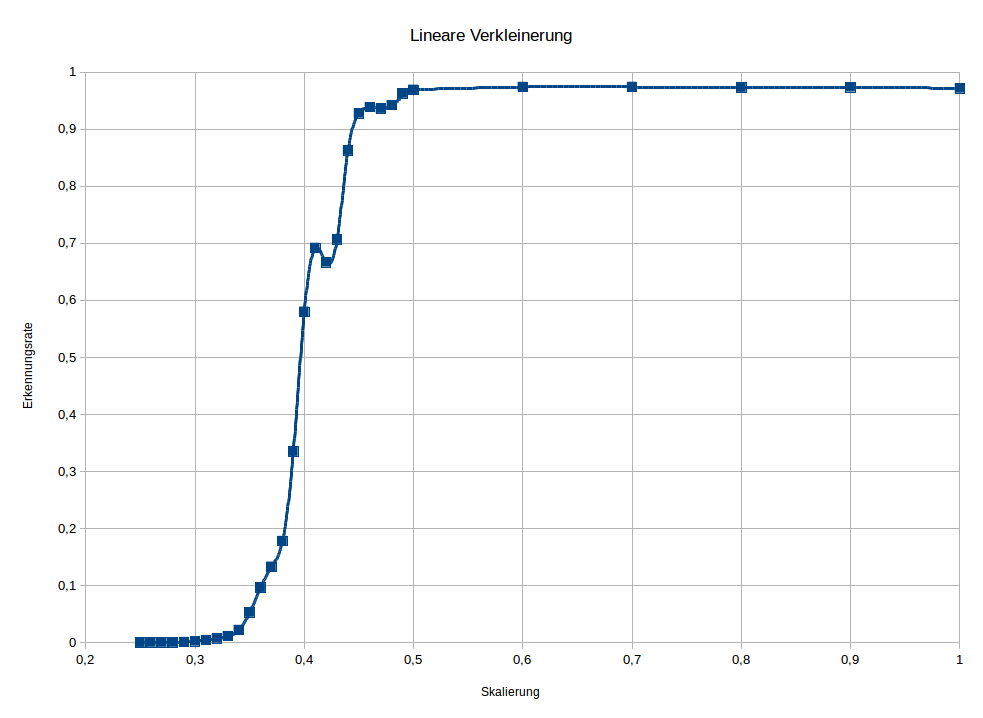
\includegraphics[width=0.5\linewidth]{img/lineare_Verkleinerung}
	\caption{Die Bilder aus Labeled Faces in the Wild \cite{database_Face} wurden mit den Faktor auf der X-Achse linear verkleinert und die Erkennungsrate Y-Achse abgebildet}
	\label{img_lineareverkleinerung}
\end{figure}
Es ist zu erkennen, dass die Wahrscheinlichkeit auf eine erfolgreiche Detektion ab $0.5$, also etwa Gesichert mit 47 Pixel Breite, rapide abnimmt. Bei der verwendeten Kamera \autoref{hardware} entspricht dies einer Distanz von etwa $4.5m$.\\
Bei der maximalen Distanz auf der gearbeitet werden soll $(8.5m)$ ergibt sich eine Gesichtsgröße von etwa 22 Pixel, das einer Skalierung von 0.25 entspricht. Bei dieser Bildgröße ist keine Detektion möglich, siehe \autoref{img_lineareverkleinerung}.
\subsection{verschiedenen Skalierungesverfahren}
Um auf den gewünschten Distanzen arbeiten zu können, wird der jeweilige Bereich Hochskaliert. Dazu wird das Ursprüngliche Bild $(250\times 250)$ linear um den angegebene Faktor verkleinert und anschließend mit den angegebenen Verfahren auf $300\times 300$ wieder vergrößert. Die Wahrscheinlichkeit auf eine Detektion ist in \autoref{img_hochskalliern} abgebildet.\\
\begin{figure}
	\centering
	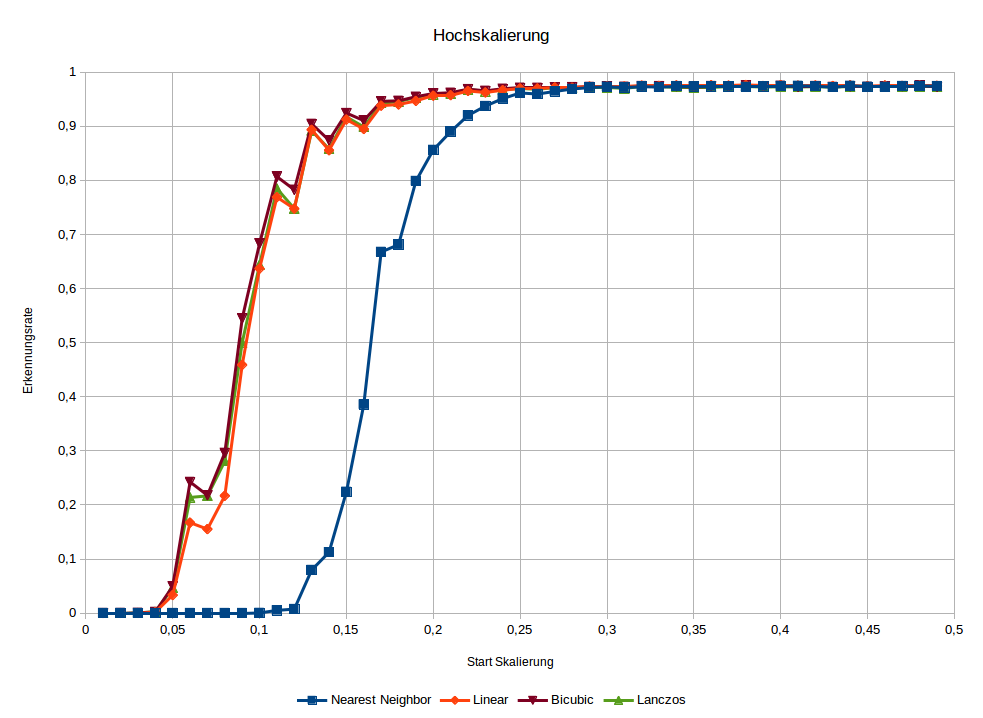
\includegraphics[width=0.5\linewidth]{img/Hochskalliern}
	\caption{Die Bilder aus Labeled Faces in the Wild \cite{database_Face} wurden mit den Faktor auf der X-Achse linear verkleinert und mit den verschiedenen Verfahren wieder vergrößert \autoref{scale_Algos}. Aufgetragen gegen die Detektionswahrscheinlichkeit.
	Nearest-Neighbor (blau), Linear (rot), Bicubic (braun), Lanczos (grün)}
	\label{img_hochskalliern}
\end{figure}
Es ist zu erkennen das durch die Vergrößerung, Gesichter in Bereichen die normal nicht erkennbar sind, bestimmbar werden. Als das ungeeignetste Verfahren hat sich Nearest-Neighbor herausgestellt, siehe blaue Linie \autoref{img_hochskalliern}. Die anderen haben sehr ähnliche Ergebnisse, nur das Lineare Verfahren ist etwas schlechter. Dennoch werden die Anforderungen, einer Detektion auf Gesichtern von 22 Pixel (Skalierung 0.25) von allen erfüllt.\\
Ausgehend vom Skalierungsfaktor des Linearen-, Bicubic- und Lanczos-Verfahren wären mit der verwendeten Kamera auch Distanzen bis zu $14m$ möglich. Allerdings ist das Bild durch die Verkeilung  deutlich besser als Originalaufnahmen, da Pixelrauschen nicht vorhanden ist.
\subsection{Auswirkung von Pixelrauschen}
Durch Aufnahme eines Schwarzbildes der Actioncam zeigt sich, dass das Pixelrauschen recht hoch ist, siehe \autoref{img_noishight}. Das Rauschen hat keine Normalverteilung, sondern es besteht aus kleinen Bereiche, die den selben fehlerhaften Farbwert besitzen.
\begin{figure}
	\centering
	\fbox{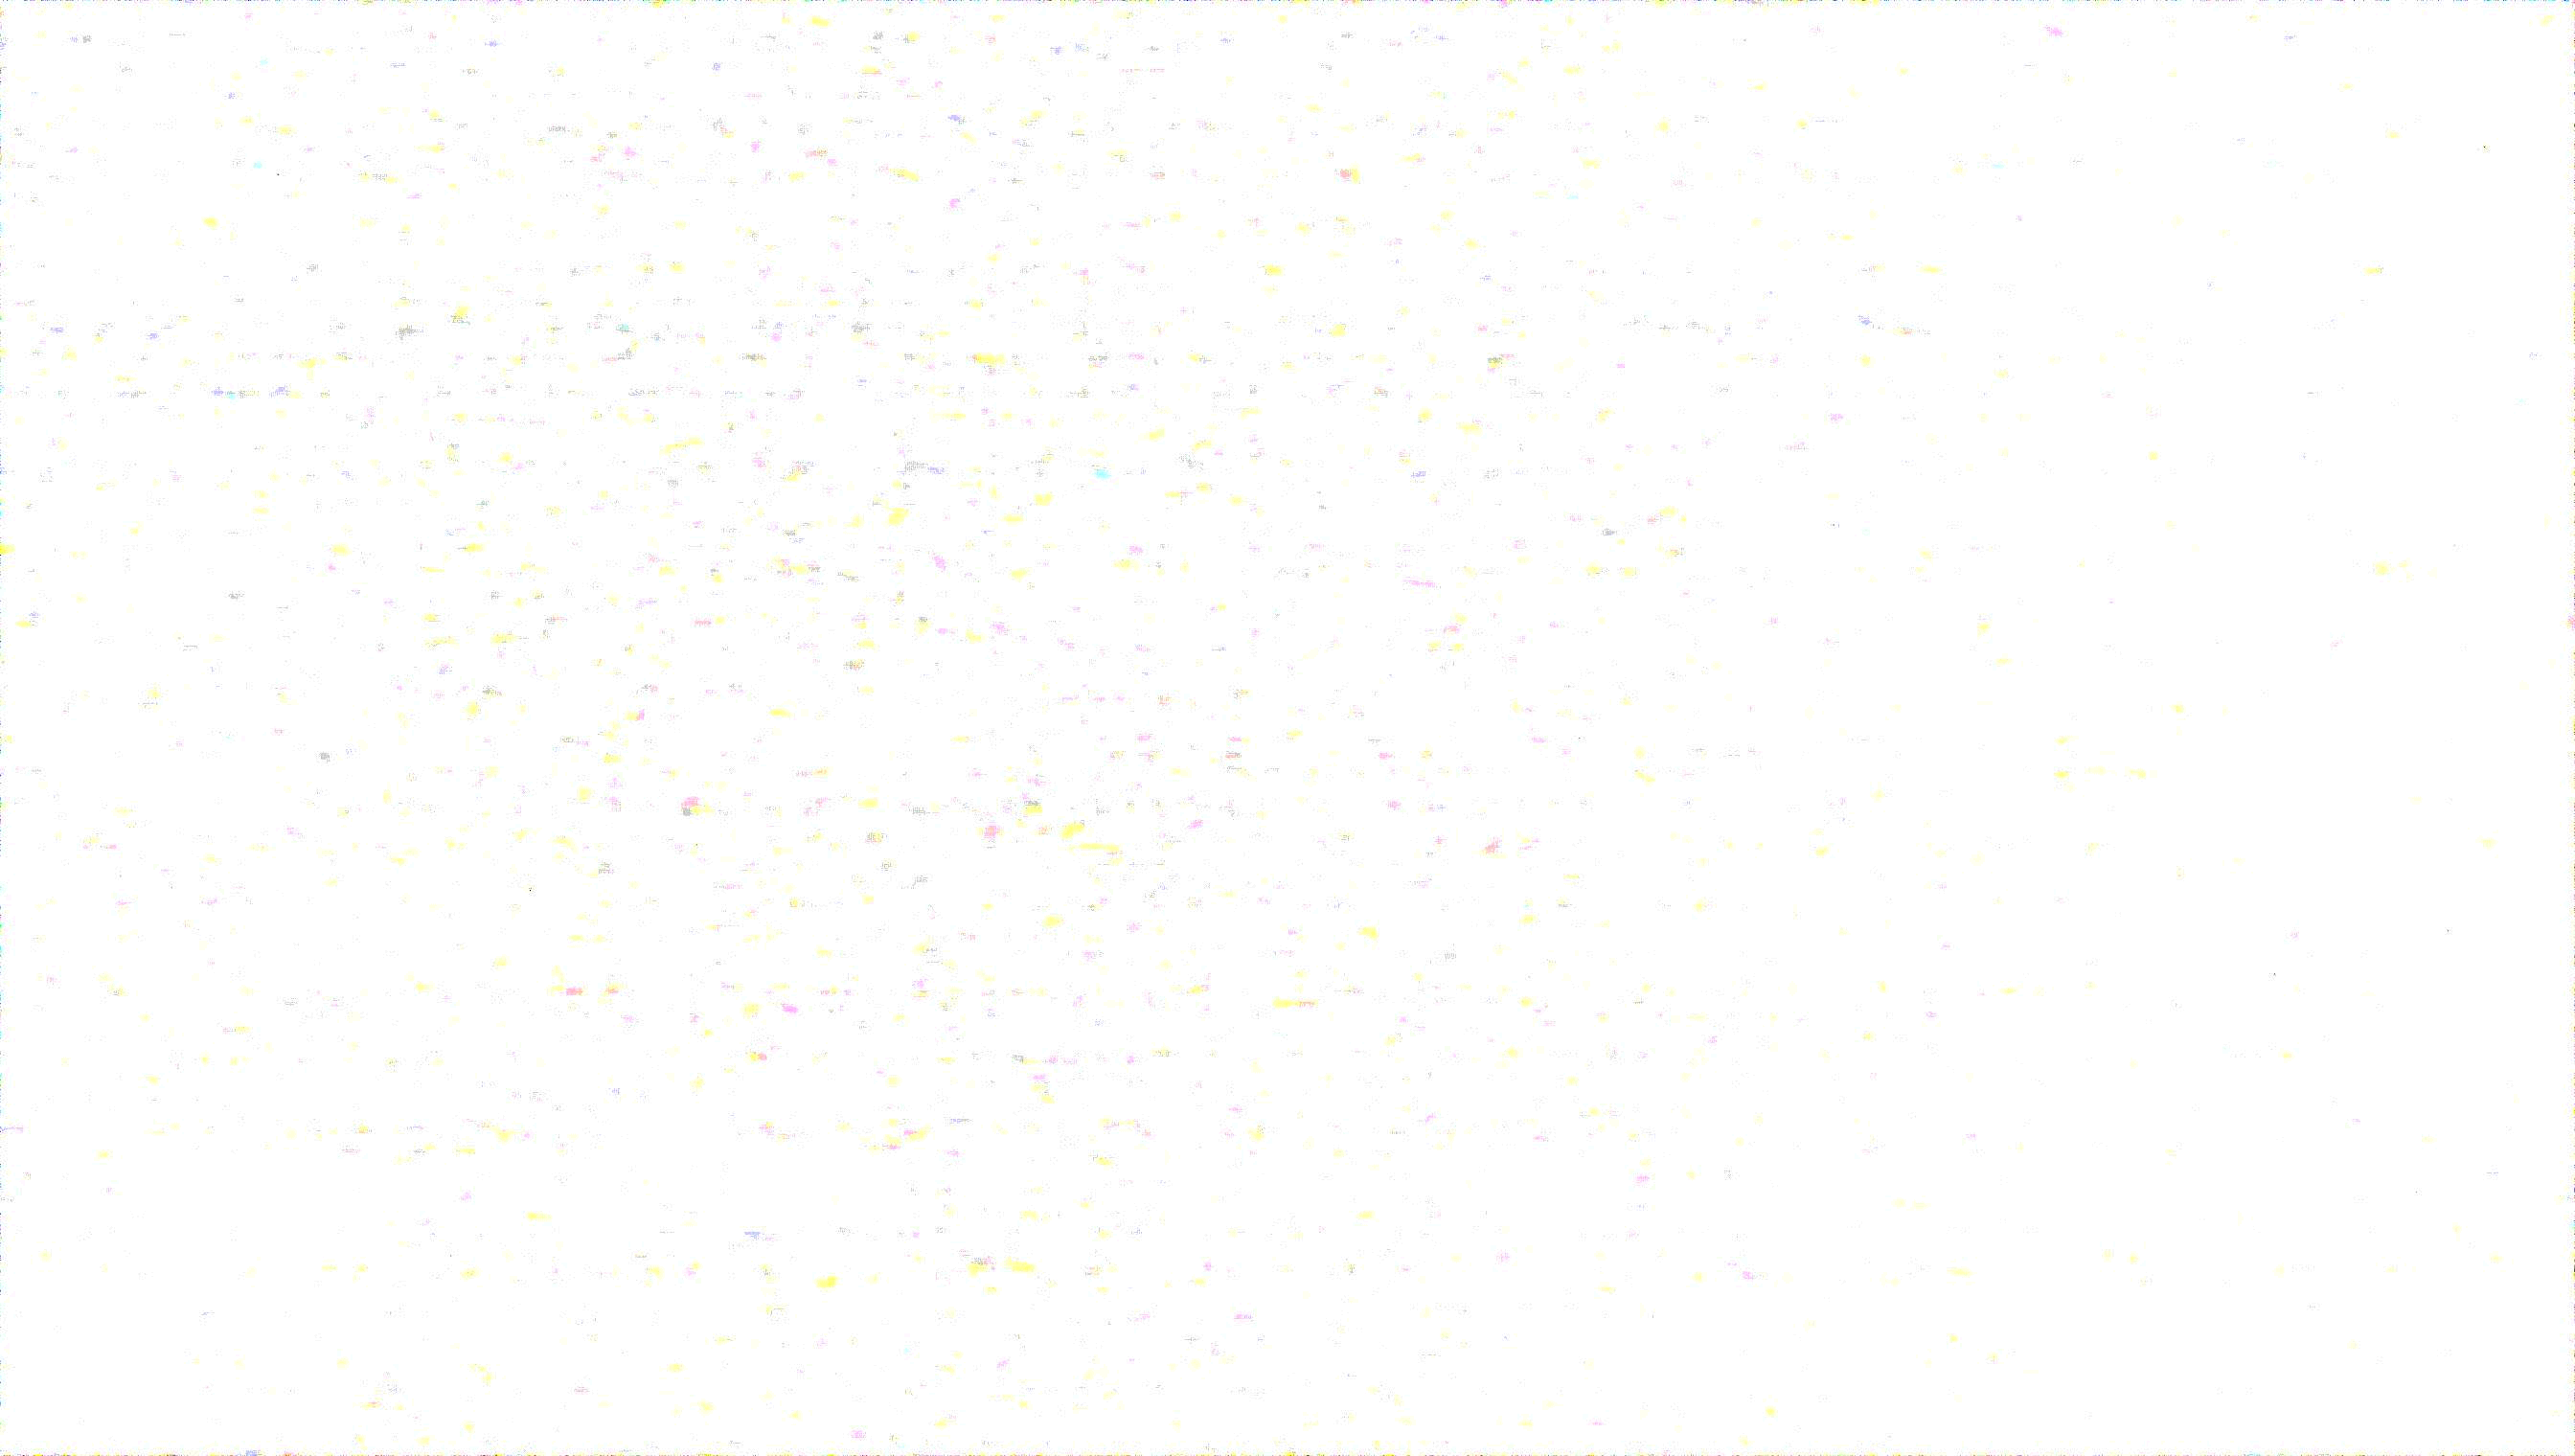
\includegraphics[width=1\linewidth]{img/NoisHight}}
	\caption{Aufnahme eines Schwarz-Bildes $(2688\times 1520)$ der Actioncam um den Faktor 7 verstärkt und invertiert.}
	\label{img_noishight}
\end{figure}

\subsection{To Do}
\begin{itemize}
	\item Patch Experts und Optimierungsfunktionen CLM
	\item Auswirkung von Pixelrauschen
	\begin{itemize}
		\item Rauschen der Actioncam bestimmen\\
		Done
		\item Simulation des Rauschens\\
		Add Gaußverteilung auf Image 
	\end{itemize}
\item Distanzen
\item Winkel
\item Auswerten der Messung
\item Wann ELSE
\item Mittlung Ergebnis / Landmarks
\item Zuverlässigkeit mit Farbkorrektur
\end{itemize}
\section{Fehleranalyse}
Mit entsprechend hochauflösenden Kameras, können auch bessere Resultate auf größeren Distanzen erzielt werden. Gerade die Bestimmung der Blickrichtung auf großer Distanz ist meist nicht möglich, da die Augenpartie viel zu klein für eine Berechnung ist. So bleibt meist nur die Gesichtsorientierung mit ihr natürlichen Ungenauigkeit.\\
Da Bewegung erlaubt ist, passiert es immer wieder, dass Teile des Gesichtes verdeckt werden, durch Hände beim Melden, andere Schüler oder dem Lehrer selbst, der vor der Kamera steht oder sich der Kopf zu weit wegdreht und das Tracking scheitert. Aber auch die Frisuren spielen eine Rolle, da dadurch diese einige Landmarks verdeckt werden können, wie z.B. die Augenbrauen, und das Gesicht nicht erkannt wird .

%%%%%%%%%%%%%%%%%%%%%%%%%%%%%%%%%
% Das Literaturverzeichnis      %
%%%%%%%%%%%%%%%%%%%%%%%%%%%%%%%%%

\addcontentsline{toc}{chapter}{Literaturverzeichnis}
% Dadurch werden die Zitate mit abgekürzten Namen der Autoren generiert.
\bibliographystyle{alpha}
\bibliography{Quellenverzeichnis}
\end{document}